
\documentclass[twoside]{article}
\usepackage{eadh2026}
\begin{document}

%===============================================================
% Title and authors

\title{Geographic Citation Insularity in Digital Humanities:\ A Bibliometric Analysis Using OpenAlex} % Abstract title

\author[1]{anonymous \orcid{anon}}

\affil[1]{anonymous}

\titlerunning{Citation Insularity in DH}      % Shortened title to be displayed in header
\authorrunning{anonymous}       % Shortened list of authors to be displayed in header

\maketitle   
\thispagestyle{empty}


%===============================================================
% Introduction

\section{Introduction}
Digital Humanities (DH) positions itself as an inherently international and interdisciplinary endeavour. Yet scholars have long questioned whether the field's citation practices reflect this aspiration. \textcite{fiormonte2012} argues that DH scholarship is shaped by Anglophone and Western European power structures, while \textcite{galina2014} documents the geographic and linguistic unevenness of DH research output. \textcite{risam2019} extends this critique to show how digital knowledge production reproduces global inequalities.

These arguments have been primarily corroborated by qualitative analysis and descriptive counts of conference submissions \parencite{weingart2017}, with only two bibliometric analyses \parencite{spinaci2022,tang2017}. In this paper, we update and extend these large-scale bibliometric studies, focusing on whether DH citation networks are geographically insular---that is, whether scholars preferentially cite work from their own country, and if so, how much this exceeds what would be expected given the distribution of global DH output.

This paper addresses three research questions: (1)~To what extent do DH scholars cite works from their own country? (2)~How does observed citation insularity compare to a null model based on country-level publication shares? (3)~How have these patterns changed over time (2007--2025)?

%===============================================================
% Introduction

\section{Data and Methods}
\subsection{Corpus Construction}

We built a DH corpus using a twofold strategy following \textcite{spinaci2022}. First, we retrieved all works published since 2000 in the 19 journals classified as ``Exclusively DH'' in the Spinaci et al.\ curated list. Second, we retrieved all works whose title or abstract contains the phrase ``digital humanities,'' regardless of venue. After deduplication, the core corpus comprises approximately 17,600 works. All data were retrieved from \href{https://openalex.org/}{OpenAlex} \parencite{priem2022} using \texttt{openalexR} \parencite{aria2024}.

For each work, we extracted all author-affiliated countries using the OpenAlex \texttt{authorships.countries} field, applying full counting (each country associated with any author is credited). We then extracted all outgoing references and batch-fetched their country metadata. This yielded 58,655 citation-level records where both the citing and cited work have known country affiliations, spanning 63 countries with at least 100 citations each.

\subsection{Conference Corpus}

To compare against a major non-journal venue, we processed the \textit{Index of Digital Humanities Conferences} \parencite{weingart2020}, a relational extract of conference abstracts maintained by Carnegie Mellon University. Author countries were obtained by joining the extract's authorship, affiliation, and institution tables, resolving institution countries to ISO codes through an auditable crosswalk. Unlike the journal corpus, conference abstracts carry no machine-readable citation links, so we reconstructed the citation network from text: reference strings were extracted from each abstract's full text, segmented one reference per line, and parsed with the AnyStyle reference parser to isolate cited-work titles. Because the OpenAlex search API timed out on a large fraction of these queries, we resolved references \textit{offline} against a local copy of the OpenAlex works snapshot, matching on DOI, then exact title, then a high-threshold fuzzy title match (Jaro--Winkler $\geq 0.95$), and accepting only high-confidence matches to favour precision over recall. This resolved 11{,}645 references ($\sim$27\%); after the further requirement that cited works carry country metadata, roughly 5{,}000 conference citation edges entered the analysis. Each conference was tagged by series, distinguishing the international ADHO annual conference (and its predecessor series) from regional venues, so that the two are not conflated. The same insularity measures and null model (below) were applied identically to both corpora.

\subsection{Insularity Measures}

A citation is \textit{insular} when authors cite works produced in their own country — a form of geographic self-citation. More formally, a citation from work $C$ (with country set $S_C$) to work $R$ (with country set $S_R$) is classified as \textit{insular} under two definitions: (1)~\textit{Any overlap}: $S_C \cap S_R \neq \emptyset$; (2)~\textit{Majority rule}: $|S_C \cap S_R| / |S_C| > 0.5$. The self-citation rate (SCR) for country $c$ is the share of its citations that are insular.

\subsection{Null Model}

To distinguish genuine preference from base-rate effects---the US produces more DH works, so US authors will cite US works more often by chance---we computed an expected SCR for each country equal to its share of the cited-works pool. We then tested whether observed SCR significantly exceeds this expectation using a permutation test ($n = 1{,}000$), randomly reassigning country labels to cited works while preserving the citation graph structure.

\subsection{Sensitivity Analysis}

We ran the full analysis on three corpus tiers: (1)~\textit{Exclusively}, only works from the 19 exclusively DH journals; (2)~\textit{Core}, "Exclusively DH" plus keyword-matched works (our primary analysis); (3)~\textit{All}, Core plus works from 17 ``Significantly DH'' journals. Results were substantively identical across tiers.


%===============================================================
\section{Results}

\subsection{Overall Insularity and Temporal Trends}

Across all 58,655 citations, 28\% are insular under the any-overlap definition and 19\% under majority rule. However, this aggregate masks a clear temporal decline: overall SCR fell from approximately 40\% in 2007--2009 to 27\% in 2022--2025 (see \autoref{fig:temporal}). This suggests that DH citation networks have become progressively more international over the past two decades.

% Figure 1: Temporal trend
\begin{figure}[t]
  \centering
      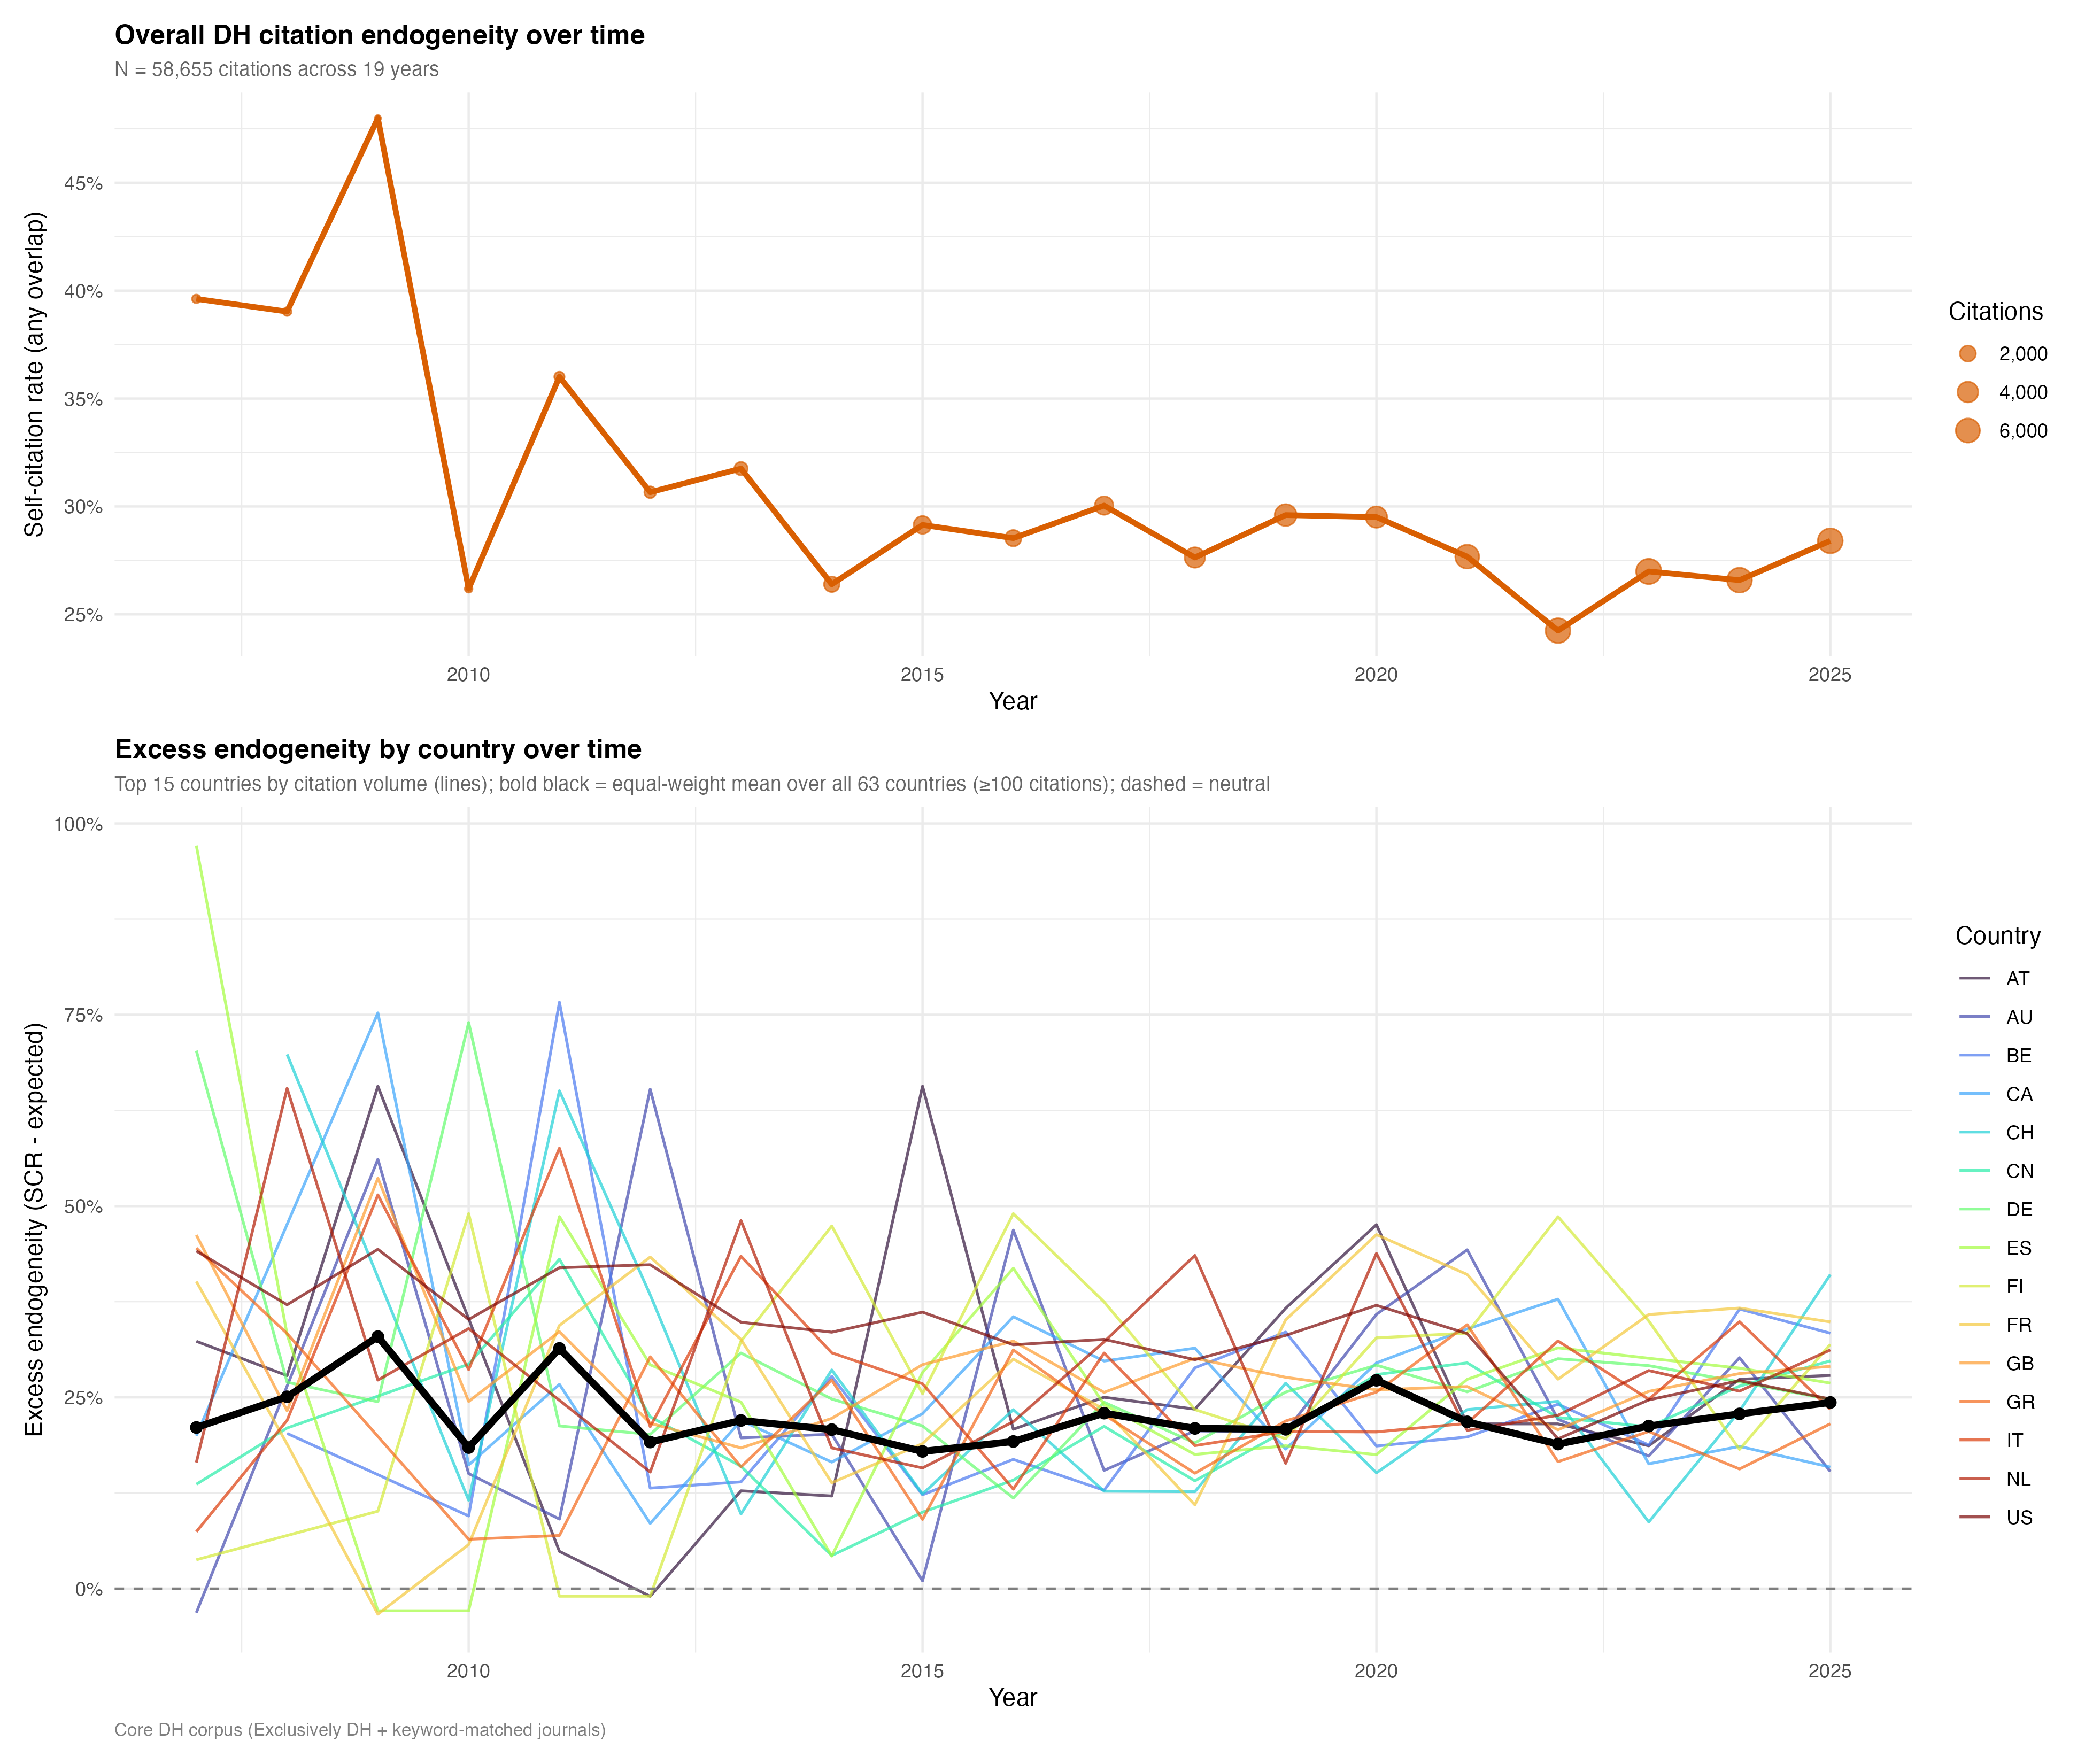
\includegraphics[width=0.85\textwidth]{figures/fig3_temporal_trends.png}
  \caption{Overall DH citation insularity (any overlap) over time, 2007--2025. Point size proportional to annual citation volume ($N = 58{,}655$ total). Core DH corpus (Exclusively DH journals + keyword-matched works).}
  \label{fig:temporal}
\end{figure}

A linear trend analysis reveals that only the United States shows a statistically significant decline ($\beta = -1.0$ percentage points/year, $p < 0.001$, $R^2 = 0.68$). Most other countries exhibit negative slopes that do not reach significance, likely due to greater year-to-year volatility in smaller samples.

\subsection{Country-level Excess Insularity}

\autoref{tab:countries} presents insularity metrics for the 15 largest DH-producing countries. Every country's observed SCR significantly exceeds the null-model expectation ($p < 0.05$ for all 30 countries with $\geq 100$ citations), confirming that geographic self-citation in DH is a universal and statistically robust phenomenon.

This bilateral structure is visualised in \autoref{fig:heatmap}, which maps excess citation---observed minus expected share---for every pair among the top 30 countries. The diagonal is uniformly positive (every country cites itself more than chance), while the off-diagonal reveals where countries cite each other above or below expectation. Most countries cite the United States \textit{below} the rate its share of global DH output would predict, spending their citations disproportionately on themselves instead.

% Figure 2: Excess citation heatmap
\begin{figure}[t]
  \centering
      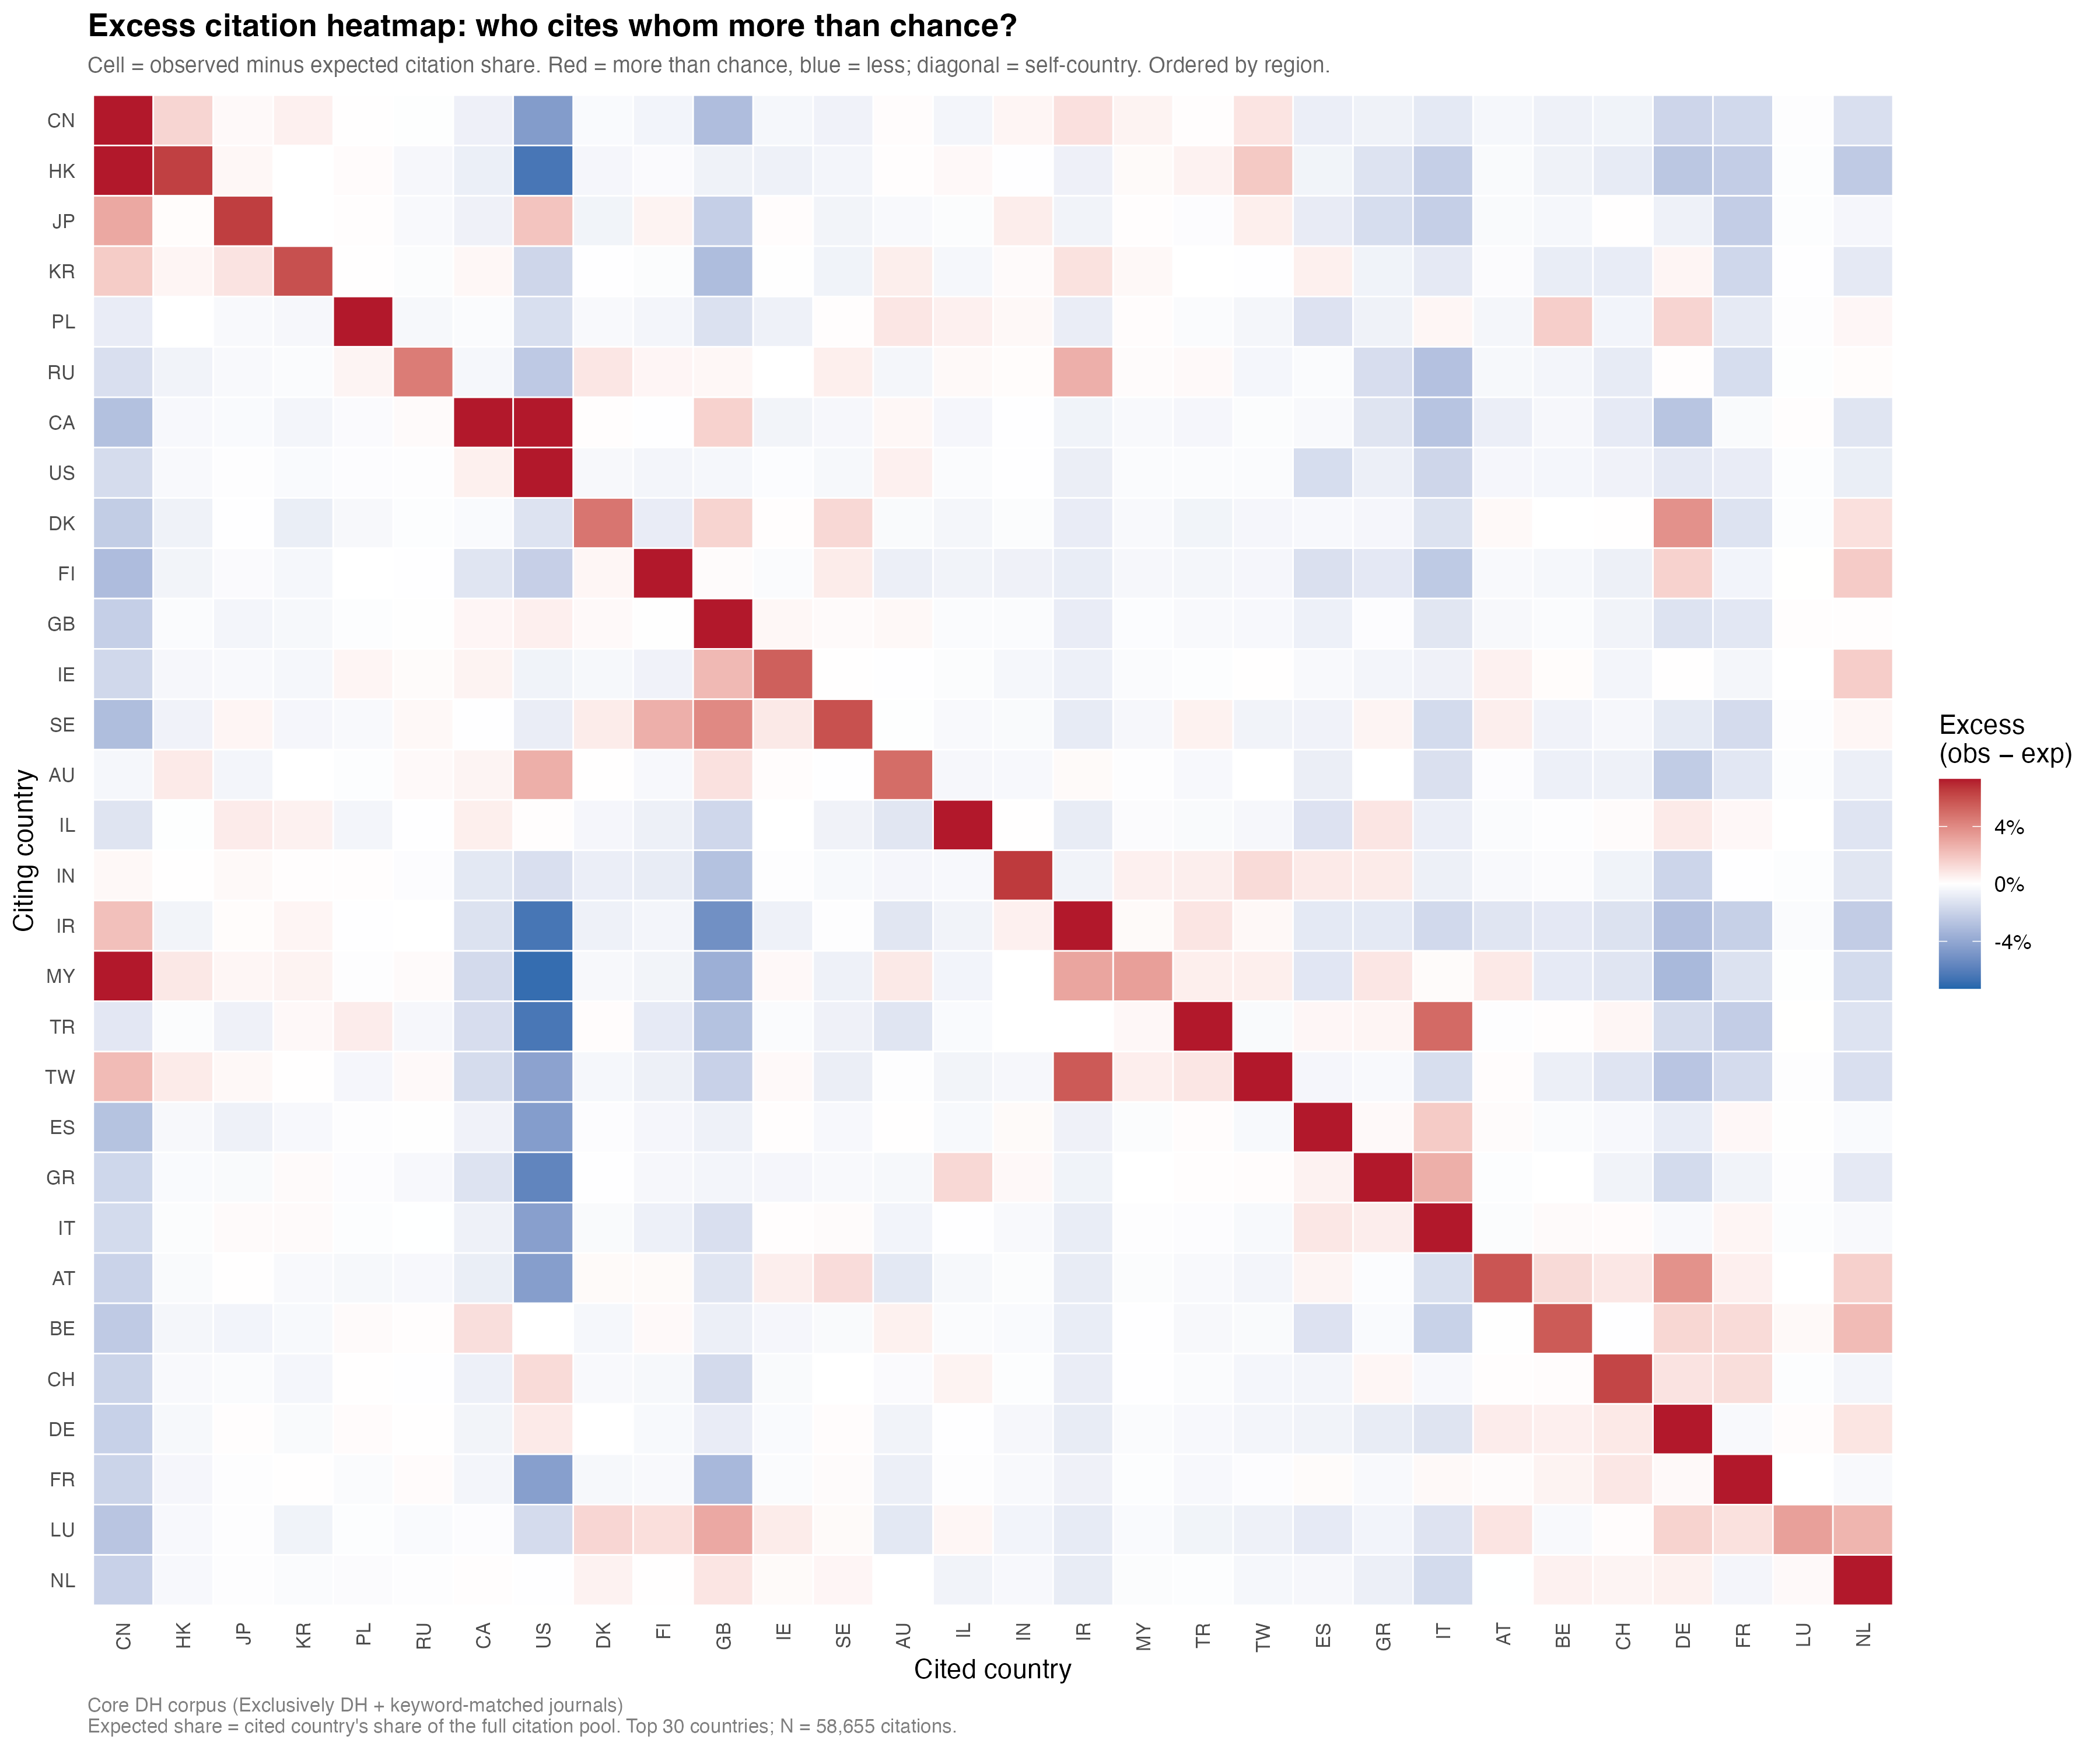
\includegraphics[width=0.95\textwidth]{figures/fig2_citation_heatmap.png}
  \caption{Excess citation heatmap for the top 30 DH-producing countries: each cell is the observed minus expected citation share (expected = cited country's share of the full citation pool). Red indicates citing more than chance, blue less; the diagonal is self-country insularity. Rows and columns are ordered by geographic region. Core DH corpus.}
  \label{fig:heatmap}
\end{figure}

\begin{table}[t]
\center
\small
\begin{tabular}{lrrrrrr}
\toprule
Country & $N_{\mathrm{cit}}$ & SCR\textsubscript{obs} & SCR\textsubscript{exp} & Excess & Ratio & $p$ \\
\midrule
US & 9{,}646 & .602 & .290 & .312 & 2.1 & $<$.001 \\
GB & 8{,}111 & .384 & .115 & .269 & 3.3 & $<$.001 \\
CN & 6{,}449 & .296 & .040 & .256 & 7.4 & $<$.001 \\
DE & 6{,}146 & .318 & .060 & .258 & 5.3 & $<$.001 \\
IT & 5{,}884 & .305 & .041 & .264 & 7.5 & $<$.001 \\
FR & 3{,}294 & .355 & .033 & .322 & 10.7 & $<$.001 \\
ES & 3{,}185 & .285 & .029 & .256 & 9.9 & $<$.001 \\
NL & 3{,}172 & .300 & .035 & .265 & 8.5 & $<$.001 \\
CA & 2{,}611 & .283 & .038 & .244 & 7.4 & $<$.001 \\
CH & 2{,}512 & .228 & .016 & .212 & 14.2 & $<$.001 \\
GR & 2{,}091 & .218 & .009 & .208 & 22.9 & $<$.001 \\
AU & 1{,}775 & .287 & .031 & .255 & 9.1 & $<$.001 \\
FI & 1{,}489 & .308 & .010 & .298 & 31.2 & $<$.001 \\
BE & 1{,}445 & .229 & .011 & .218 & 20.1 & $<$.001 \\
AT & 1{,}414 & .279 & .010 & .269 & 27.9 & $<$.001 \\
\bottomrule
\end{tabular}
\caption{Insularity metrics for the 15 largest DH-producing countries (core corpus, any-overlap definition). SCR\textsubscript{obs}: observed self-citation rate. SCR\textsubscript{exp}: expected rate under the null model. Excess: observed minus expected. Ratio: observed divided by expected. $p$-values from 1{,}000-permutation test.}
\label{tab:countries}
\end{table}

The \textit{insularity ratio} (observed/expected) reveals a striking pattern: smaller DH-producing countries show far higher ratios. Finland (ratio 31.2), Austria (27.9), and Greece (22.9) cite themselves many times more than their share of global DH output would predict, whereas the US (ratio 2.1), which produces the most DH work, has a lower ratio despite the highest absolute excess (31.2 percentage points). This indicates that geographic self-citation is especially concentrated in countries with smaller but cohesive national DH communities.

\subsection{Bridge Scholars}

We identified 668 authors meeting minimum thresholds (3+ DH works, 10+ outgoing citations) and computed their citation entropy (Shannon) across countries. The most geographically diverse scholars cite works from over 40 countries. However, the proportion of bridge scholars (top-quartile entropy) among active DH authors has declined since a peak around 2010, coinciding with the overall growth of the field and the entry of less internationally connected researchers.

\subsection{Conference Proceedings}

To test whether the declining journal trend extends to a major non-journal venue, we replicated the analysis on the \textit{Index of DH Conferences} (Carnegie Mellon), recovering references from abstract full text and resolving them against a local OpenAlex snapshot. Coverage is necessarily partial---a reference must be parseable, present in OpenAlex, and carry country metadata---yielding 11{,}645 resolved references ($\sim$27\%) across the conference corpus. We restrict the conference analysis to the international ADHO annual conference (and its predecessor series), so the comparison is not confounded by mechanically national venues.

\autoref{fig:conf} contrasts insularity over time at the ADHO conference against the journal baseline. The conference rate is high and broadly \textit{flat} ($\sim$42\% any-overlap), in marked contrast to the steady journal decline. The German-language DHd series---the only regional series with sufficient resolved citations to measure---tracks the ADHO level closely ($\sim$40\%). The conference venue thus shows no sign of the internationalisation visible in journals; if anything, the live, co-located nature of conferences appears to sustain geographically concentrated citation.

% Figure 3: Conference vs journal temporal
\begin{figure}[t]
  \centering
      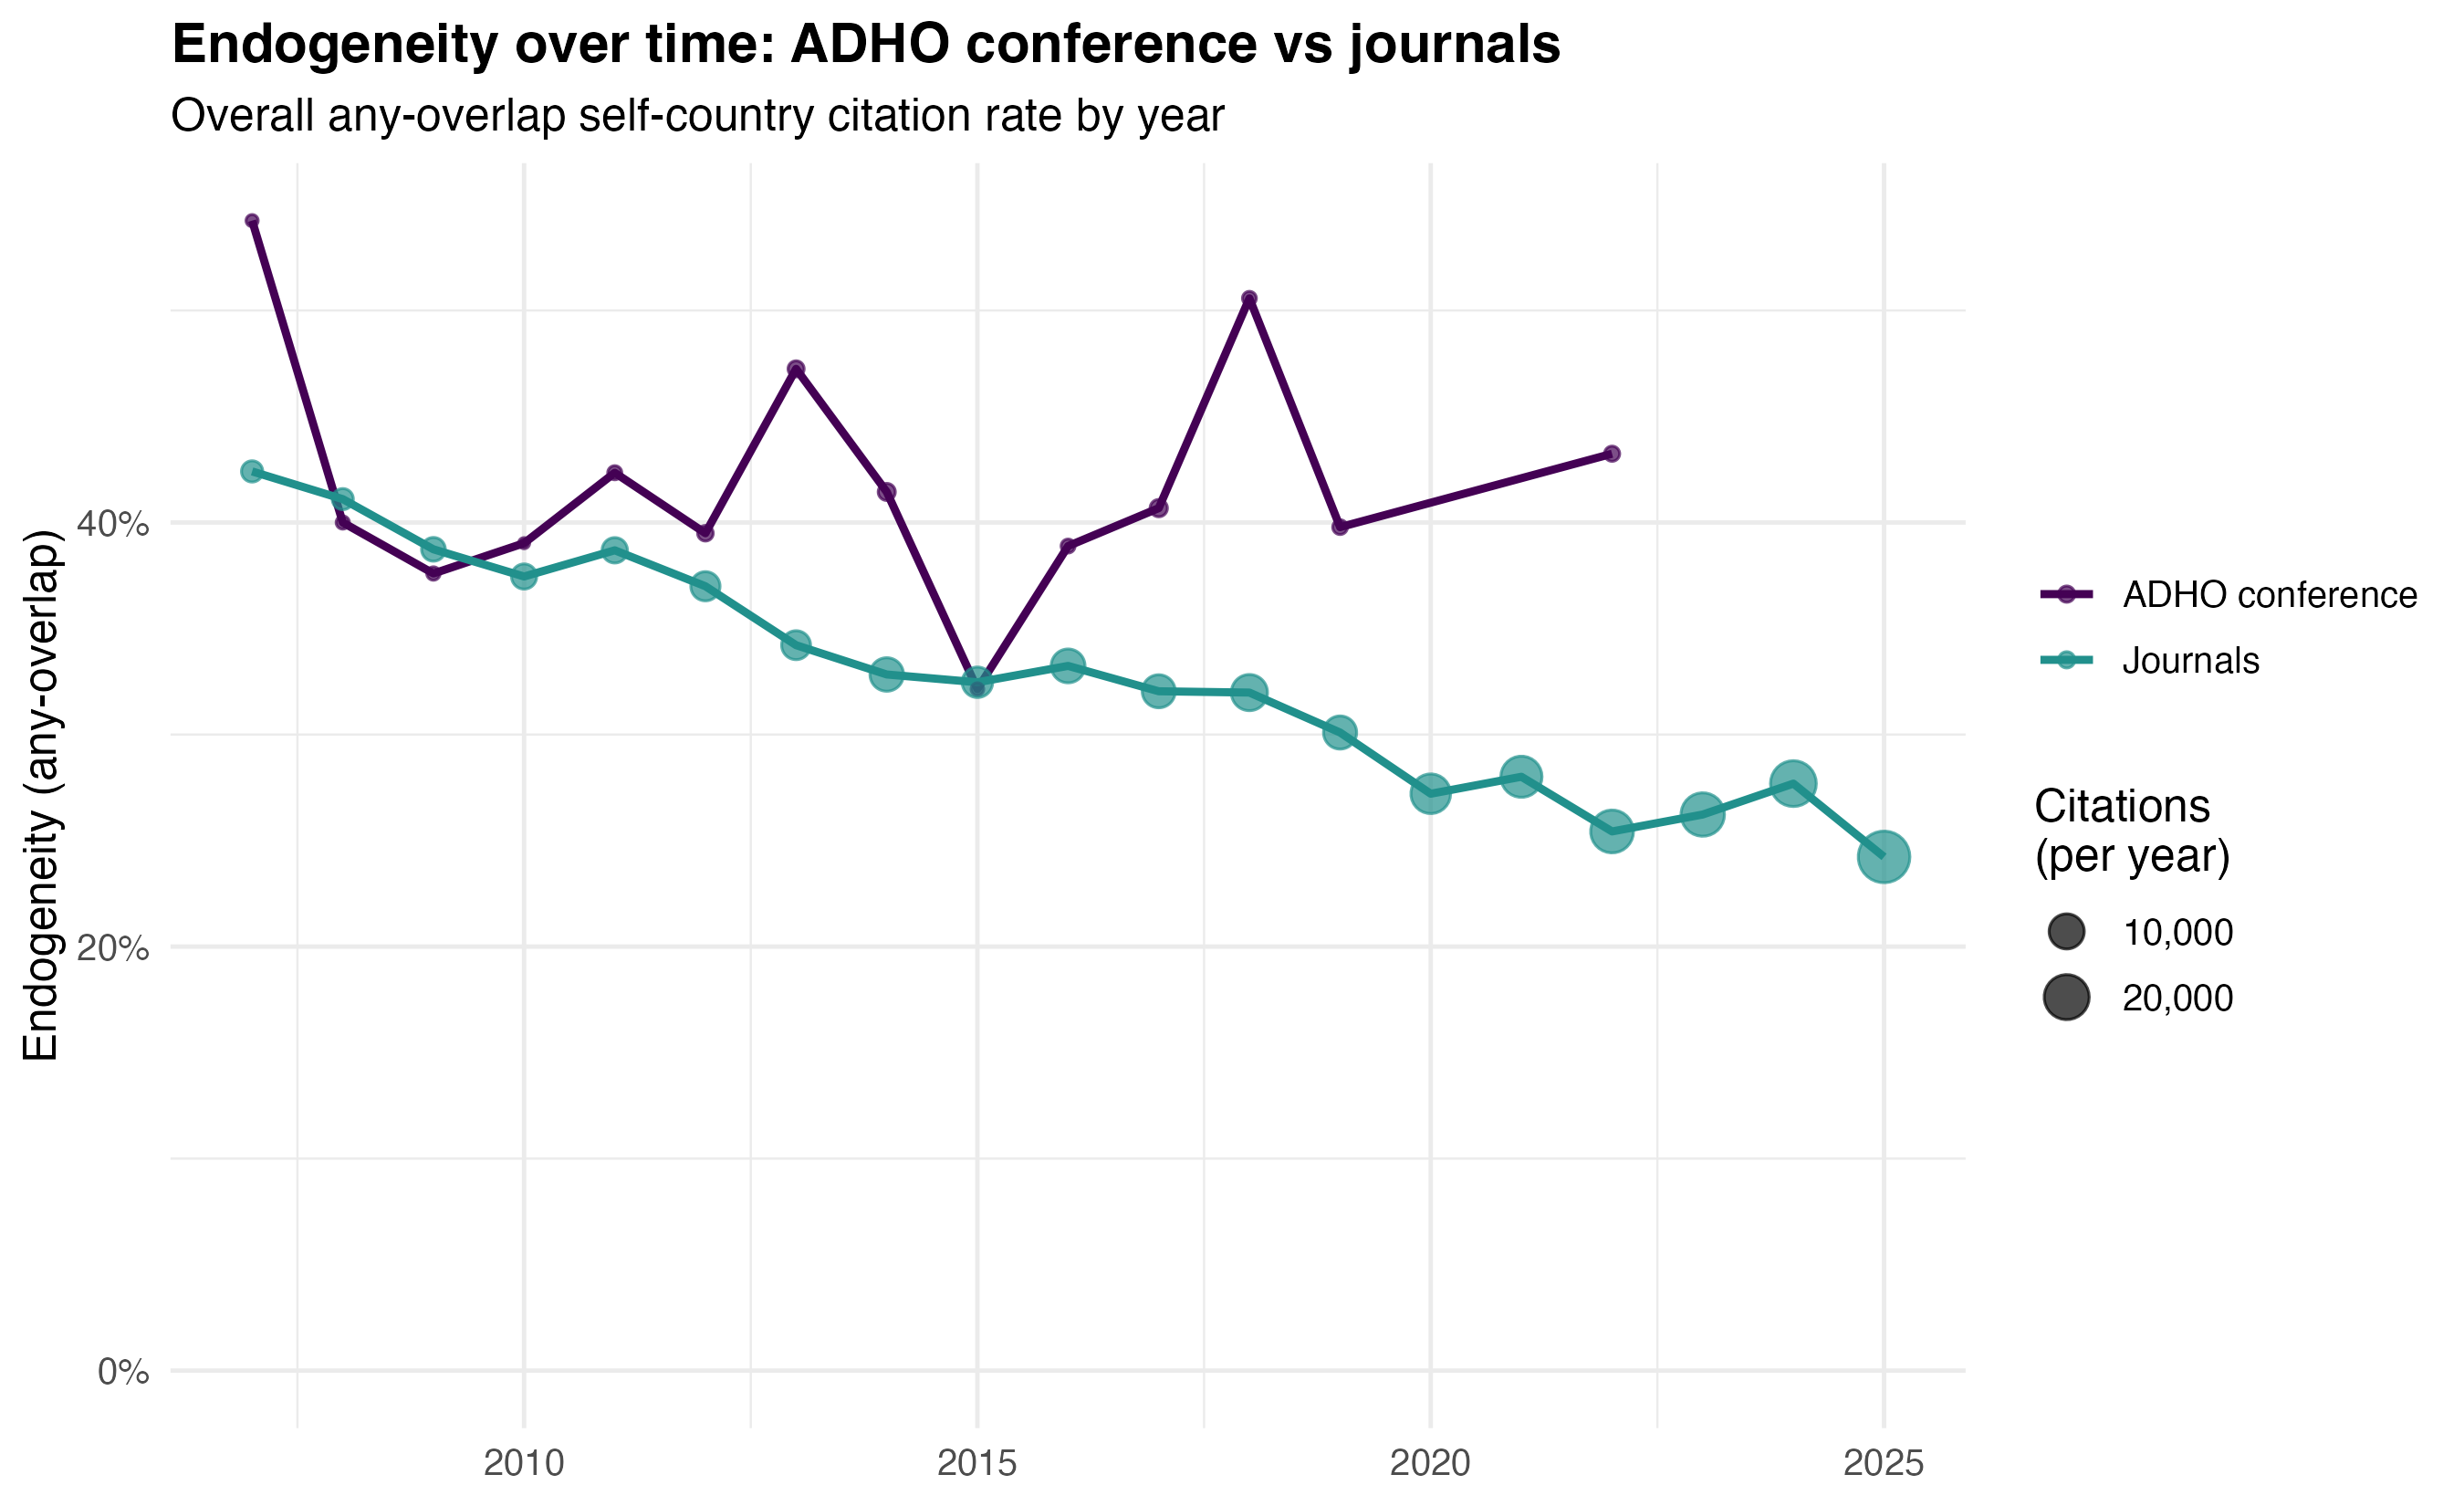
\includegraphics[width=0.85\textwidth]{figures/fig9_conf_vs_journal_temporal.png}
  \caption{Insularity over time (any overlap): conference series ($\geq 50$ resolved citations) versus the journal corpus (dashed black baseline). Point size proportional to annual citation volume; conference counts are far smaller, so yearly points are noisier. Conference figures derive from a coverage-filtered subset and are indicative.}
  \label{fig:conf}
\end{figure}


%===============================================================
\section{Discussion and Conclusion}

Our analysis demonstrates that geographic citation insularity in DH is universal, statistically significant, and structurally embedded: every country with sufficient data cites itself more than chance alone would predict. At the same time, the declining temporal trend---from 40\% to 27\% over two decades---suggests that DH is gradually becoming more internationally integrated, consistent with the field's globalizing ambitions.

The insularity ratio results have important implications: while the US and UK dominate absolute citation volumes, it is smaller national communities (Finland, Austria, Greece) where geographic insularity is most amplified relative to expectations. This may reflect the role of national-language scholarship, local institutional networks, and the concentration of DH activity in a small number of research groups.

Several limitations should be noted. Our primary corpus is journal-centric; we extend it to ADHO conference proceedings, but conference references are recovered from abstract full text and only partially resolvable, so the conference results rest on a coverage-filtered subset and should be read as indicative rather than exhaustive. Only the ADHO and DHd series carry enough resolved citations to measure, so the per-series conference comparison is effectively limited to those two venues. The keyword-search component may over-represent works that self-identify as ``digital humanities'' while missing computational studies published in disciplinary venues. Full counting inflates the role of multi-country collaborations. Finally, country is an imperfect proxy for linguistic and cultural communities \parencite{nyhan2014,tang2017}.

Ongoing work will extend the analysis by benchmarking DH against other humanities and social science fields (History, Literature, Sociology, Political Science) to determine whether DH's insularity patterns are distinctive or typical of academic disciplines more broadly. Code and data are available at: \texttt{[repository anonymized for submission]}.


%===============================================================
% Bibliography
\printbibliography

\end{document}
